\documentclass{article}
\usepackage{hyperref}
\usepackage{graphicx}
\usepackage{geometry}

 \geometry{
 a4paper,
 left=20mm,
 right=20mm,
 top=20mm,
 }
 
\hypersetup{
    colorlinks,
    citecolor=black,
    filecolor=black,
    linkcolor=black,
    urlcolor=black
}

\begin{document}

    \section{Subsystems}
    
    \subsection{Notification Subsystem}
    
    \subsubsection{Overview}
    
    The notifications module provides notifications to system users regarding
    particular system updates that a user would like to be notified about through
    some medium external to the application.
    
    \subsubsection{UML Diagrams}
    
    \begin{figure}[h!]
        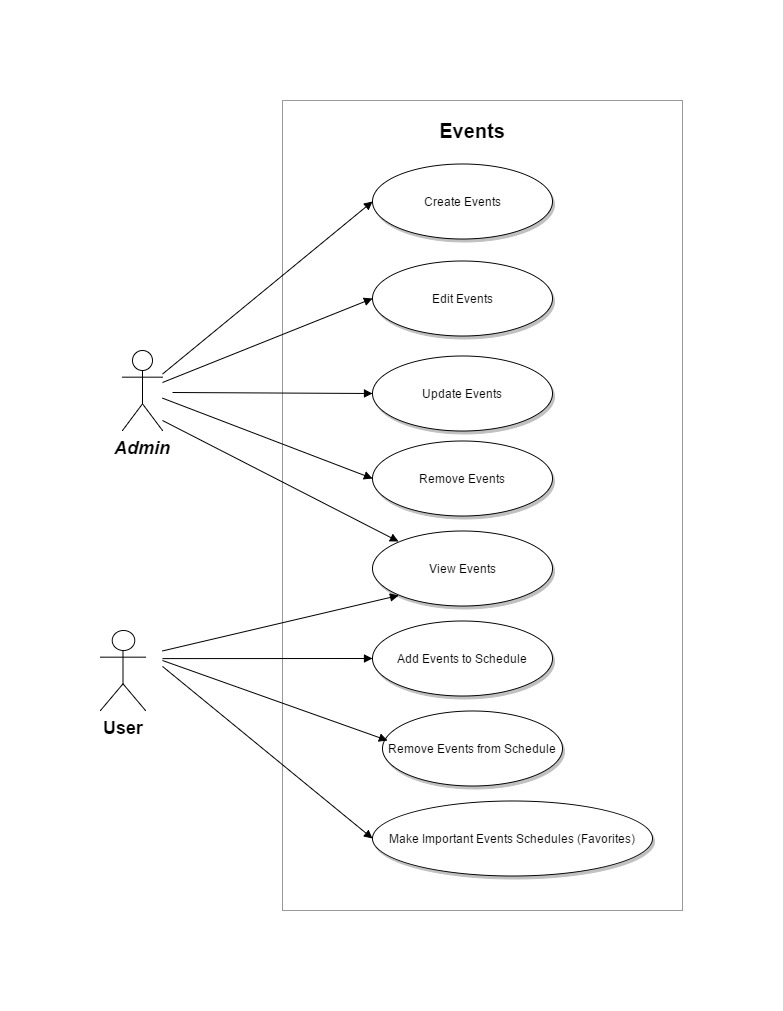
\includegraphics[width=\textwidth]{Images/EventUC.jpg}
    \end{figure}
    Events Use Case Diagram
    
    \mbox{}\\
    \bigskip
    \clearpage
    
    \begin{figure}[h!]
      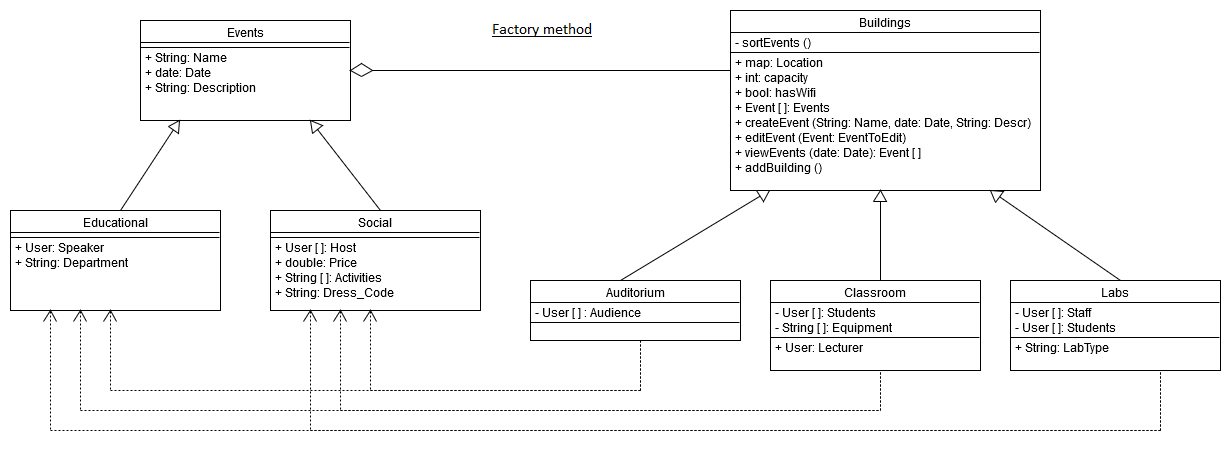
\includegraphics[width=\textwidth]{Images/ClassDiagramEvents.png}
    \end{figure}
    Notification Class Diagram
    
    \begin{flushleft}
    
        For the notifications subsystem the observer design pattern came to light, as this pattern allows objects to change state and all of its dependents follow suit. This allows a notification state to be used that can update whether or not a notification needs to be sent out. In this case the push method of observer was used. Also evident is the template design pattern that uses the concrete observers to redefine the way in which the notifications are sent. Notifying modules are also given the flexibility to decide which medium/s are used for the notification.
        
        \bigskip
        
        There are methods in the Send Email and Send SMS classes that allow users to be added to the user lists for the notifications to either or both of these mediums. There is also provision for more notification mediums to be added in the future and these can be attached to the Notify class. Should a notification medium be unavailable it can be detached from the Notify class until it is available. The Notify class can be called from any other module that would like to request a notification to be sent out to users which allows for modularity.
        
        \bigskip
        Notify: Subject
        
        Send Notification: Observer(Observer) / Abstract Method(Template)
        
        Send Email: Concrete Observer1(Observer) /Concrete Method(Template)
        
        Send SMS: Concrete Observer2(Observer) / Concrete Method(Template)
    
    \end{flushleft}
    
    \mbox{}\\
    \bigskip
    \clearpage
    
    \begin{figure}[h!]
        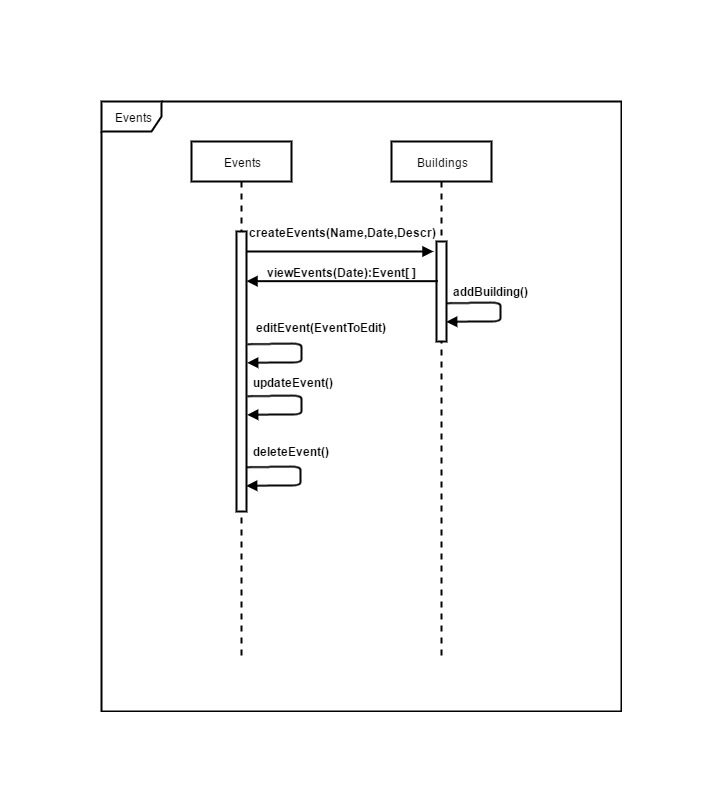
\includegraphics[width=\textwidth]{Images/EventsSequence.jpg}
    \end{figure}
    Notification Sequence Diagram
    
    \mbox{}\\
    \bigskip
    \clearpage
    
    \begin{figure}[h!]
        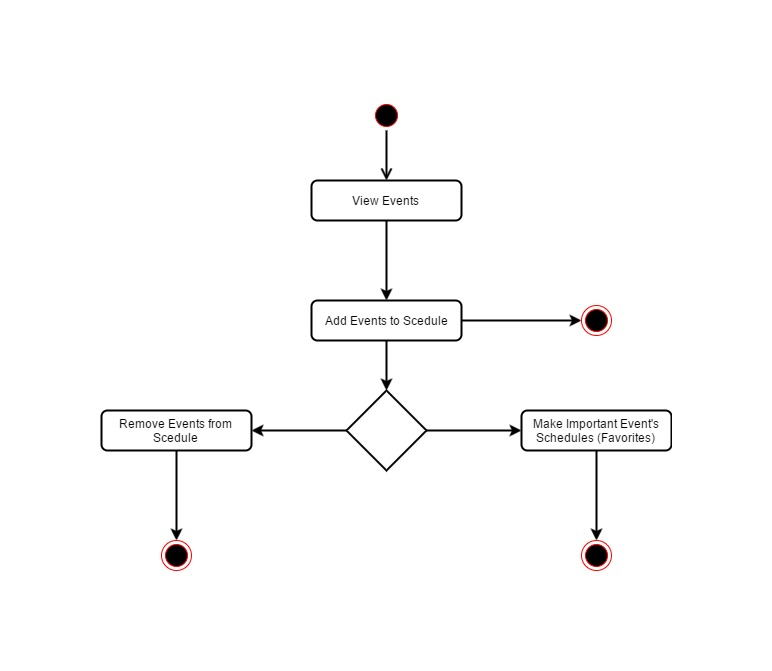
\includegraphics[width=\textwidth]{Images/ActivityDiagramUser.jpg}
    \end{figure}
    Add User Activity Diagram
    
    \mbox{}\\
    \bigskip
    \clearpage
    
    \begin{figure}[h!]
        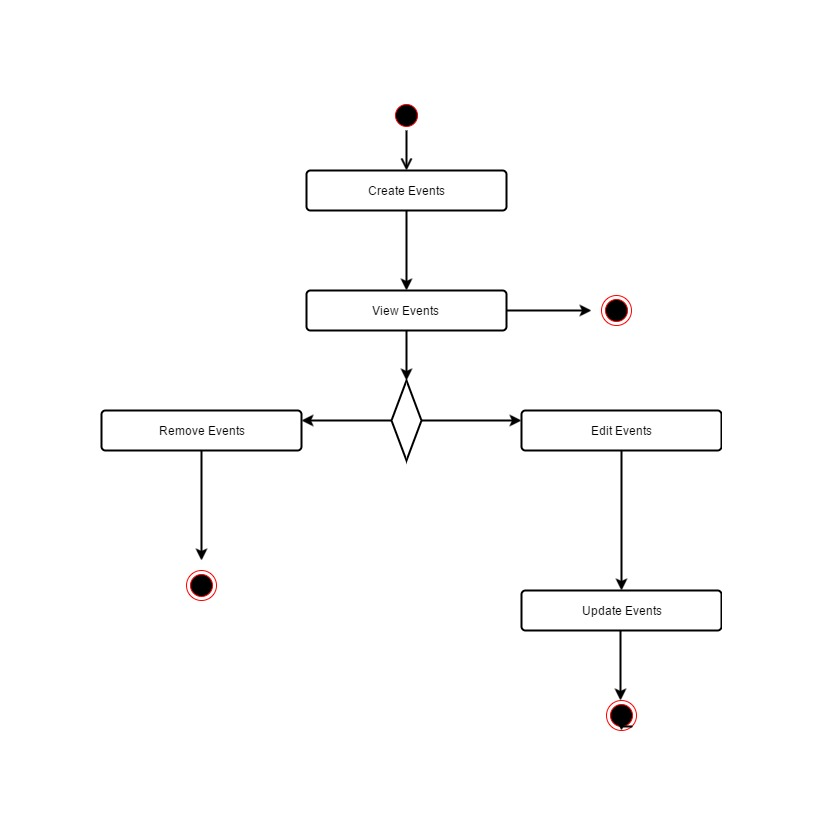
\includegraphics[width=\textwidth]{Images/ActivityDiagramAdmin.jpg}
    \end{figure}
    Send Notification Activity Diagram
    
    \mbox{}\\
    \bigskip
    \clearpage
    
    \begin{figure}[h!]
        \begin{center}
            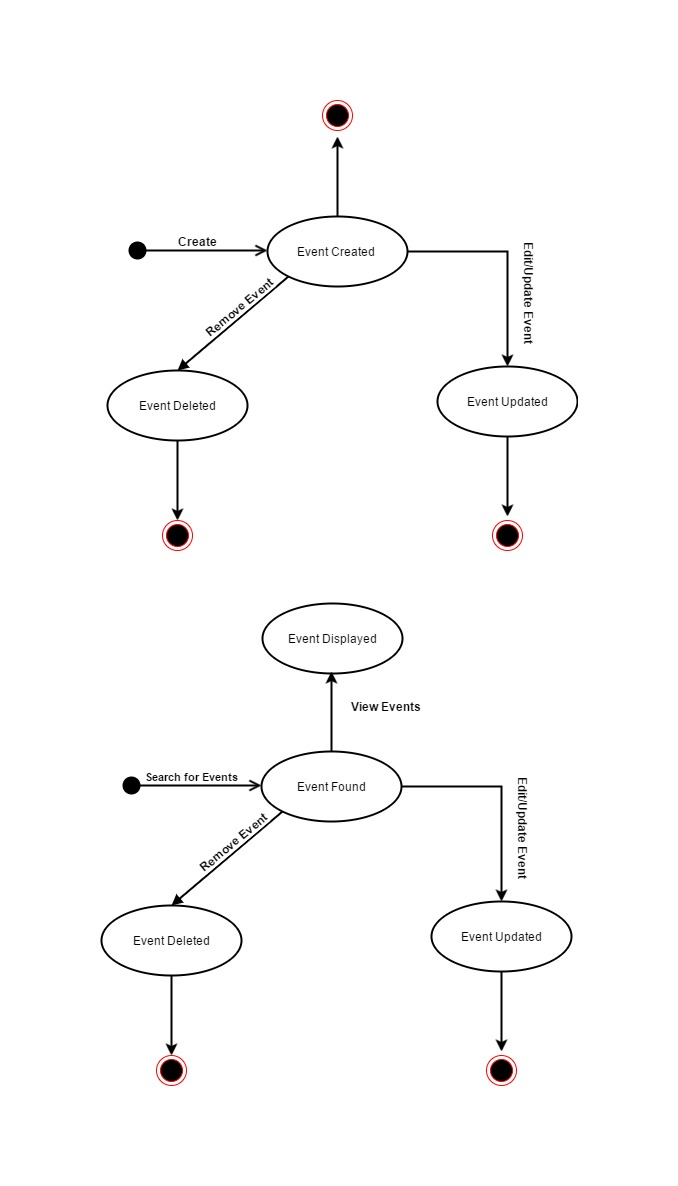
\includegraphics[width=0.6\textwidth]{Images/StateDiagramEvent.jpg}
        \end{center}
    \end{figure}
    Notification State Diagram
    
    \mbox{}\\
\end{document}
